\documentclass{article}
\usepackage{array}
\usepackage[column=0]{cellspace}
\setlength\cellspacetoplimit{6pt}
\setlength\cellspacebottomlimit{6pt}
\usepackage{graphicx} % Required for inserting images
\usepackage{amsmath}
\usepackage{amssymb}
\usepackage{amsthm}
\usepackage{amsfonts}
\usepackage{gensymb}
\newcommand{\myvec}[1]{\ensuremath{\begin{pmatrix}#1\end{pmatrix}}}
\usepackage{graphicx}
\usepackage{mathtools}

\newcommand{\mydet}[1]{\ensuremath{\begin{vmatrix}#1\end{vmatrix}}}
\providecommand{\brak}[1]{\ensuremath{\left(#1\right)}}
\providecommand{\norm}[1]{\left\lVert#1\right\rVert}
\let\vec\mathbf

\title{MathConstruction}

\begin{document}

\section{NCERT 12.10.5.9}

Find the position vector of a point R which divides the line joining two points P and Q whose Position Vectors are $2\overrightarrow{a}+\overrightarrow{b}$ and $\overrightarrow{a}-3\overrightarrow{b}$ externally in the ratio $1:2$.Also, Show that P is the mid point of the line segment QR  \\
\textbf{Solution:}
let us assume a and b and the given ratio is
\begin{table}[h]
    \centering
    \begin{tabular}{|c|c|}
        \hline
        \textbf{Symbol} & \textbf{Value} \\
        \hline
        $\vec{a}$ & $\myvec{1\\-3}$ \\
        \hline
        $\vec{b}$ & $\myvec{0\\2}$ \\
        \hline
        $k$ & $2$ \\
        \hline
    \end{tabular}
    \label{tab:mytable}
    \caption{vectors a,b and Ratio k}
\end{table}\\
using section formula
\begin{align}
    \vec{R}=\frac{\vec{Q}-k.\vec{P}}{1-k}
\end{align}\\
where P and Q depends on a and b then,
\begin{align}
	\vec{P}=(2\vec{a}+\vec{b})=2\myvec{1\\-3}+\myvec{0\\2}=\myvec{2\\-4}\\
    	\vec{Q}=(\vec{a}-3\vec{b})=\myvec{1\\-3}-3\myvec{0\\2}=\myvec{1\\-9}
\end{align}\\
where R can be calculated as 
\begin{align}
	\vec{R}=\frac{(\vec{a}-3\vec{b})-k.(2\vec{a}+\vec{b})}{1-k}
\end{align}\\
by substituting a and b values we get R as
\begin{align}
    \vec{R}=\myvec{3\\1}
\end{align}
\begin{table}[h]
    \centering
    \begin{tabular}{|c|c|}
        \hline
        \textbf{Symbol} & \textbf{Value} \\
        \hline
	$\vec{P}$ & $(2\vec{a}+\vec{b})$ \\
        \hline
	$\vec{Q}$ & $(\vec{a}-3\vec{b})$ \\
        \hline
	    $\vec{R}$ & $\frac{\vec{Q}-k.(\vec{P})}{1-k}$ \\
        \hline
    \end{tabular}
    \label{tab:mytable}
    \caption{vectors P,Q,R}
\end{table}
\begin{figure}[!ht]
    \centering
    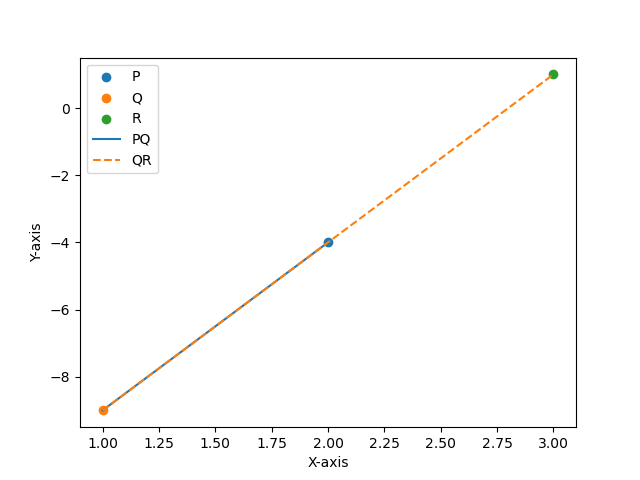
\includegraphics[width=\columnwidth]{/home/ramsai/MathComputing/codes/python/external-bisector.png}
    \caption{point vectors P,Q,R}
    \label{fig:enter-label}
\end{figure}
\end{document}
